
From the given equation, 
\begin{align}
    \vec{V} = \myvec{1 & 0 \\ 0 & -16}
    \\
    \vec{u}^{\top}\vec{V}^{-1}\vec{u}-f = 16
    \\
    \vec{c} = -\vec{V}^{-1}\vec{u}=\myvec{0 \\ 0}
    \\
    \lambda_1 = 1 , \lambda_2 = -16
\end{align}
Axes of hyperbola are given by
\begin{align}
    \sqrt{\frac{\vec{u}^{\top}\vec{V}^{-1}\vec{u}-f}{\lambda_1}} = 4\\ \sqrt{\frac{f-\vec{u}^{\top}\vec{V}^{-1}\vec{u}}{\lambda_2}} = 1
\end{align}
and the vertices are
\begin{align}
    \pm\myvec{4 \\ 0} 
\end{align}
Coordinates of the foci are given by,
\begin{align}
  \vec{F} =\pm\brak{\sqrt{\frac{(\vec{u}^T\vec{V}^{-1}\vec{u}-f)(\lambda_2-\lambda_1)}{\lambda_1\lambda_2}}}\vec{p_1} \label{quadform/2/38/b/eq:1}
\end{align}
where, $\vec{p_1} = \myvec{1 \\ 0}$ since the equation of hyperbola is in standard form.
Substituting the values in \eqref{quadform/2/38/b/eq:1} we have,
\begin{align}
    \vec{F} = \pm\myvec{\sqrt{17} \\ 0}.
\end{align}
Eccentricity of the hyperbola is given by,
\begin{align}
   e &= \frac{\sqrt{\frac{(\vec{u}^{\top}\vec{V}^{-1}\vec{u})(\lambda_2-\lambda_1)}{\lambda_1\lambda_2}}}{\sqrt{\frac{\vec{u}^{\top}\vec{V}^{-1}\vec{u}-f}{\lambda_1}}} \label{quadform/2/38/b/eq:2}
   &= \frac{\sqrt{17}}{4}.
\end{align}
upon substituting from  \eqref{quadform/2/38/b/eq:2}.
Length of the latus rectum is given by,
\begin{align}
    l &= \frac{2\brak{{\sqrt{\frac{f-\vec{u}^{\top}\vec{V}^{-1}\vec{u}}{\lambda_2}}}}^2}{\sqrt{\frac{\vec{u}^{\top}\vec{V}^{-1}\vec{u}-f}{\lambda_1}}} \label{quadform/2/38/b/eq:3}
    &= \frac{1}{2}
\end{align}
upon substituting the values in \eqref{quadform/2/38/b/eq:3}.
The above results are verified in Fig. \ref{quadform/2/38/b/Plot of standard hyperbola}.

\begin{figure}[ht]
\centering
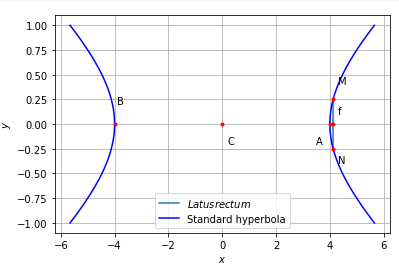
\includegraphics[width=\columnwidth]{solutions/su2021/2/38/b/hyperbola.PNG}
\caption{Plot of standard hyperbola}
\label{quadform/2/38/b/Plot of standard hyperbola}
\end{figure}

